\documentclass[11pt]{article}

\newcommand{\HWnum}{3} 
\newcommand{\StudName}{Timothy Holmes} % author
\newcommand{\CourseNum}{420}           % course number
\newcommand{\Subject}{PHY}

\usepackage{graphicx, amsmath, amssymb,fancyhdr}
\addtolength{\textwidth}{1.5in}
\addtolength{\oddsidemargin}{-2cm}
\addtolength{\evensidemargin}{-2cm}
\addtolength{\textheight}{1.6in}
\addtolength{\topmargin}{-0.7in}
\addtolength{\headsep}{-0.1in}
%\addtolength{\footskip}{-0.2in}
\pagestyle{fancy}
\cfoot{}
\lhead{\textbf{\Subject~\CourseNum~--- Homework~\HWnum}}
\rhead{\textbf{\StudName:~Page~\thepage}}

\addtolength{\parskip}{\baselineskip} % skips a line between paragraphs
\parindent 0in                        % no indent at start of paragraph

\newcommand{\dd}{\textrm{d}}
\usepackage{braket}
\usepackage{lipsum, babel}
\usepackage{blindtext}
\usepackage{graphicx}% Include figure files
\usepackage{dcolumn}% Align table columns on decimal point
\usepackage{bm}% bold math
\usepackage{listings}
\usepackage{listing}
\usepackage{supertabular}



\usepackage{color} %red, green, blue, yellow, cyan, magenta, black, white
\definecolor{mygreen}{RGB}{28,172,0} % color values Red, Green, Blue
\definecolor{mylilas}{RGB}{170,55,241}



\lstset{language=Python,%
    %basicstyle=\color{red},
    breaklines=true,%
    morekeywords={matlab2tikz},
    keywordstyle=\color{blue},%
    morekeywords=[2]{1}, keywordstyle=[2]{\color{black}},
    identifierstyle=\color{black},%
    stringstyle=\color{mylilas},
    commentstyle=\color{mygreen},%
    showstringspaces=false,%without this there will be a symbol in the places where there is a space
    numbers=left,%
    numberstyle={\tiny \color{black}},% size of the numbers
    numbersep=9pt, % this defines how far the numbers are from the text
    emph=[1]{for,end,break},emphstyle=[1]\color{red}, %some words to emphasise
    %emph=[2]{word1,word2}, emphstyle=[2]{style},    
}

\begin{document}
% -------------------------- BOD -------------------------- 

\title{Homework {\HWnum}}
\author{Timothy Holmes \\ \Subject ~ \CourseNum ~ Electrodynamics II}

\maketitle

\section*{Problem 1}

A hollow right circular cylinder of radius $b$ has its axis coincident with the $z$ axis and its ends at $z = 0$ and $z = L$. The potential on the end faces of the cylinder is zero, while the potential on the cylindrical surface is $V(\phi, z)$.

The Laplace equation in cylindrical coordinates is gave by

$$
\frac{1}{\rho} \frac{\partial}{\partial \rho} \Bigg( \rho \frac{\partial \Phi}{\partial \rho}\Bigg) + \frac{1}{\rho^{2}} \frac{\partial^{2} \Phi}{\partial \phi^{2}} + \frac{\partial^{2} \Phi}{\partial z^{2}}= 0
$$

The first step in approaching partial differential equations is to separate the variables. The variables for a cylinder are

$$
\vec{\Phi} (\vec{x}) = R(\rho)Q(\phi)Z(z)
$$

and plugging these variables into the Laplace equation gives

$$
\Bigg( \frac{d^{2}R}{d\rho^{2}} + \frac{1}{\rho}\frac{dR}{d\rho} \Bigg) \frac{1}{R} + \frac{1}{\rho^{2}} \frac{d^{2}Q}{d\rho^{2}} \frac{1}{Q} + \frac{1}{Z}\frac{d^{2}Z}{dz^{2}} = 0.
$$

The boundary conditions are at the bottom of the cylinder $z = 0$ and the top of the cylinder $z = L$, where the length of the cylinder is some length $L$. With all boundary conditions applied to the problem, the new potential can be expressed in the form 

$$
\Phi(\rho, \phi, z) = \sum_{m = 0} \sum_{n = 1} J_{m}\Big(\frac{in\pi \rho}{L}\Big) (C_{m, n} e^{im\phi} + D_{m, n} e^{-im\phi})sin\Big(\frac{n\pi z}{L} \Big).
$$

The Bessel function of the first kind is gave from the equation $I_{\nu}$. Therefore, $J_{\nu}(ix) = i^{\nu} I_{\nu}(x)$ which can be substituted into the equation above and gives

$$
\Phi(\rho, \phi, z) = \sum_{m = 0} \sum_{n = 1} i^{m} I_{m}\Big(\frac{in\pi \rho}{L}\Big) (C_{m, n} e^{im\phi} + D_{m, n} e^{-im\phi})sin\Big(\frac{n\pi z}{L} \Big).
$$

From here the final boundary condition can be applied. The potential on the cylindrical surface is $V(\phi, z)$. Therefore, we set $\Phi(\phi, z) \rightarrow V(\phi, z)$ and since $\rho$ is not included in the new potential, then set $\rho = a$. The new potential can now be expressed as 
$$
V(\phi, z) = \sum_{m = 0} \sum_{n = 1} i^{m} I_{m}\Big(\frac{in\pi a}{L}\Big) (C_{m, n} e^{im\phi} + D_{m, n} e^{-im\phi})sin\Big(\frac{n\pi z}{L} \Big).
$$

The potential needs to be multiplied by $sin$ and integrated such that

$$
\int_{0}^{L} dz \int_{0}^{2\pi} V(\phi, z)e^{-im\phi} sin\Big(\frac{n'\pi z}{L}\Big)d\phi
$$

and now the coefficients can be solved for. Where

$$
C_{m,n} = \Bigg[L\pi i^{m} I_{m}\Big(\frac{n \pi a}{L}\Big)\Bigg]^{-1} \int_{0}^{L} dz \int_{0}^{2\pi} V(\phi, z)e^{-im\phi} sin\Big(\frac{n'\pi z}{L}\Big)d\phi
$$

and $D_{m,n}$ is just the complex conjugate of $C_{m, n}$, therefore, we have $D_{m,n} = C_{m,n}^{*}$. Thus, we get the final expression 

$$
\Phi(\rho, \phi, z) = \frac{1}{L \pi} \sum_{m = 0}^{\infty} \sum_{n = 1}^{\infty} \frac{I_{m}(n\pi \rho / L)}{I_{m}(n\pi a / L)} (C_{m, n} e^{im\phi} + C_{m, n}^{*} e^{-im\phi}) sin\Big(\frac{n\pi z}{L} \Big).
$$

\clearpage

\section*{Problem 2}

Much of the previous problem can be used to solve this problem. Starting from the integral of $C_{m,n}$, there are now two integrals needed. One of those integrals will be from $-\pi/2$ to $\pi/2$. The other integral will be from $\pi/$ to $3\pi/2$. This set up as the constant looks like

$$
C_{m,n} = \int_{0}^{L} dz \int_{-\pi/2}^{\pi/2} V e^{-im\phi} sin\Big(\frac{n\pi z}{L}\Big)d\phi - \int_{0}^{L} dz \int_{-\pi/2}^{\pi/2} Ve^{-im\phi} sin\Big(\frac{n\pi z}{L}\Big)d\phi 
$$

Evaluating the integrals above we get

$$
C_{m,n} = \frac{8LV}{mn\pi} (-1)^{(m-1)/2}.
$$

Substituting the constant $C_{m,n}$ into the potential from problem 1 we get

$$
\Phi(\rho, \phi, z) = \frac{16V}{\pi^{2}} \sum_{m = 0}^{\infty} \sum_{n = 1}^{\infty} \frac{I_{m}(n\pi \rho / L)}{I_{m}(n\pi a / L)} \frac{(-1)^{(m-1)/2}}{mn}  cos(\phi m) sin\Big(\frac{n\pi z}{L} \Big).
$$


\clearpage

\section*{Problem 3}

In Jackson chapter 3, Jackson gives the solutions to $J_{\nu}(x)$ in equation 3.82 and $J_{-\nu}(x)$ in equation 3.83. To show that $J_{-m}(x) = (-1)^{m}J_{m}(x)$, equation 3.83 can be used. Equation 3.83 is gave as 

$$
J_{-\nu}(x) = \Bigg(\frac{x}{2}\Bigg)^{-\nu} \sum_{j=0}^{\infty} \frac{(-1)^{j}}{j! \; \Gamma(j - \nu + 1)} \Bigg(\frac{x}{2}\Bigg)^{2j}
$$

If $\nu$ is not an integer, then the solutions are linearly independent. If $\nu$ is an integer, then we have $\nu = m$. The equation above then can be wrote as

$$
J_{-m}(x) = \Bigg(\frac{x}{2}\Bigg)^{-m} \sum_{j=0}^{\infty} \frac{(-1)^{j}}{j! \; \Gamma(j - m + 1)} \Bigg(\frac{x}{2}\Bigg)^{2j}.
$$

When the condition $j < m$ is satisfied, the denominator component $(j - m + 1)!$ is infinite.  The starting term for the summation is $j = m$, so setting $j = k + m$ gives the result 

$$
J_{-m}(x) = \Bigg(\frac{x}{2}\Bigg)^{-m} \sum_{k = 0}^{\infty} \frac{(-1)^{(k + m)}}{(k + m)! \; \Gamma(k + m - m + 1)} \Bigg(\frac{x}{2}\Bigg)^{2(k + m)} = 
\Bigg(\frac{x}{2}\Bigg)^{-m} \sum_{k = 0}^{\infty} \frac{(-1)^{(k + m)}}{(k + m)! \; k!} \Bigg(\frac{x}{2}\Bigg)^{2(k + m)} 
$$

Therefore, we get 

$$
J_{-m}(x) = (-1)^{m}J_{m}(x)
$$

\clearpage

\section*{Problem 4}

The figures were generated using the program in the Appendix

\begin{figure}[htp]
    \centering
    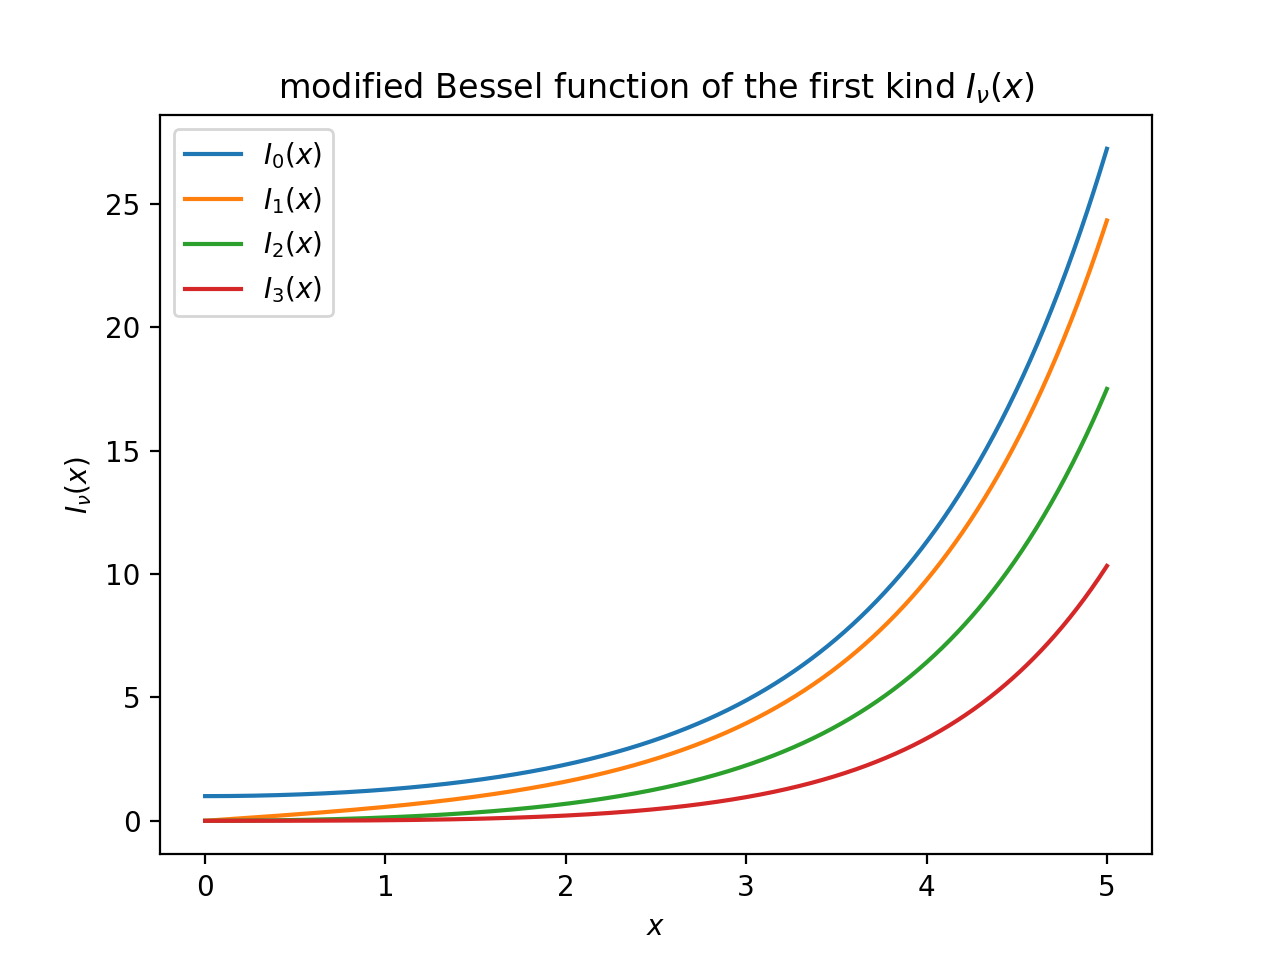
\includegraphics[width=10cm]{Figure_1.png}
    \caption{modified Bessel function of the first kind $I_{\nu}(x)$.}
    \label{fig:img}
\end{figure}


\begin{figure}[htp]
    \centering
    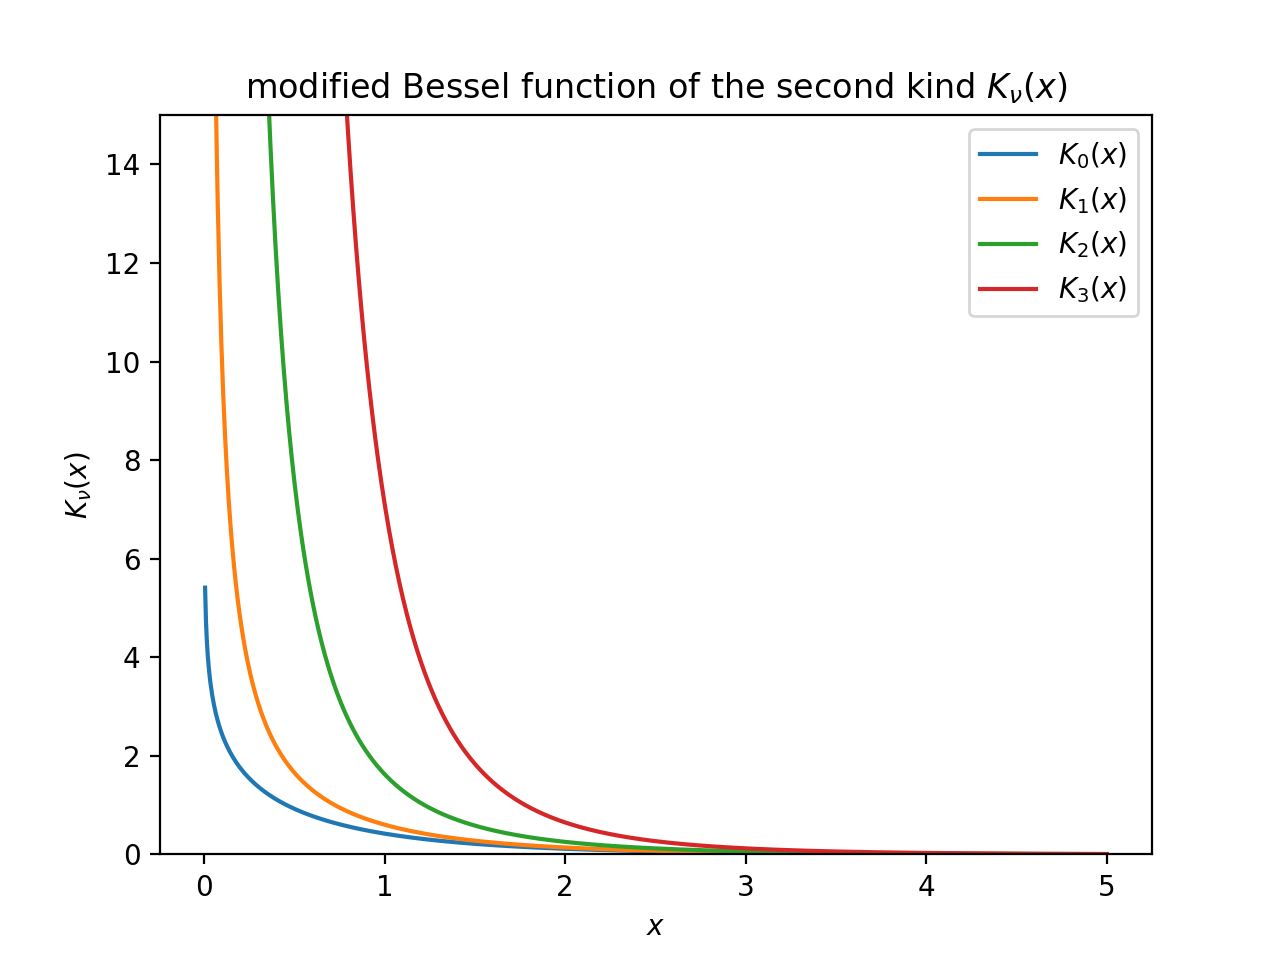
\includegraphics[width=10cm]{Figure_2.png}
    \caption{modified Bessel function of the second kind $K_{\nu}(x)$.}
    \label{fig:img}
\end{figure}


\clearpage

\section*{Appendix}

%\subsection*{Python modified Bessel program}
\lstinputlisting{homework_3.py}

\subsection*{Julia modified Bessel program}
\lstinputlisting{homework_3.jl}

\clearpage


% -------------------------- EOD -------------------------- 
\end{document}